\begin{figure}[htbp]

\centering
\begin{subfigure}[t]{0.49\textwidth}
\captionsetup{labelformat=empty}

\caption{\textbf{AAPL}}
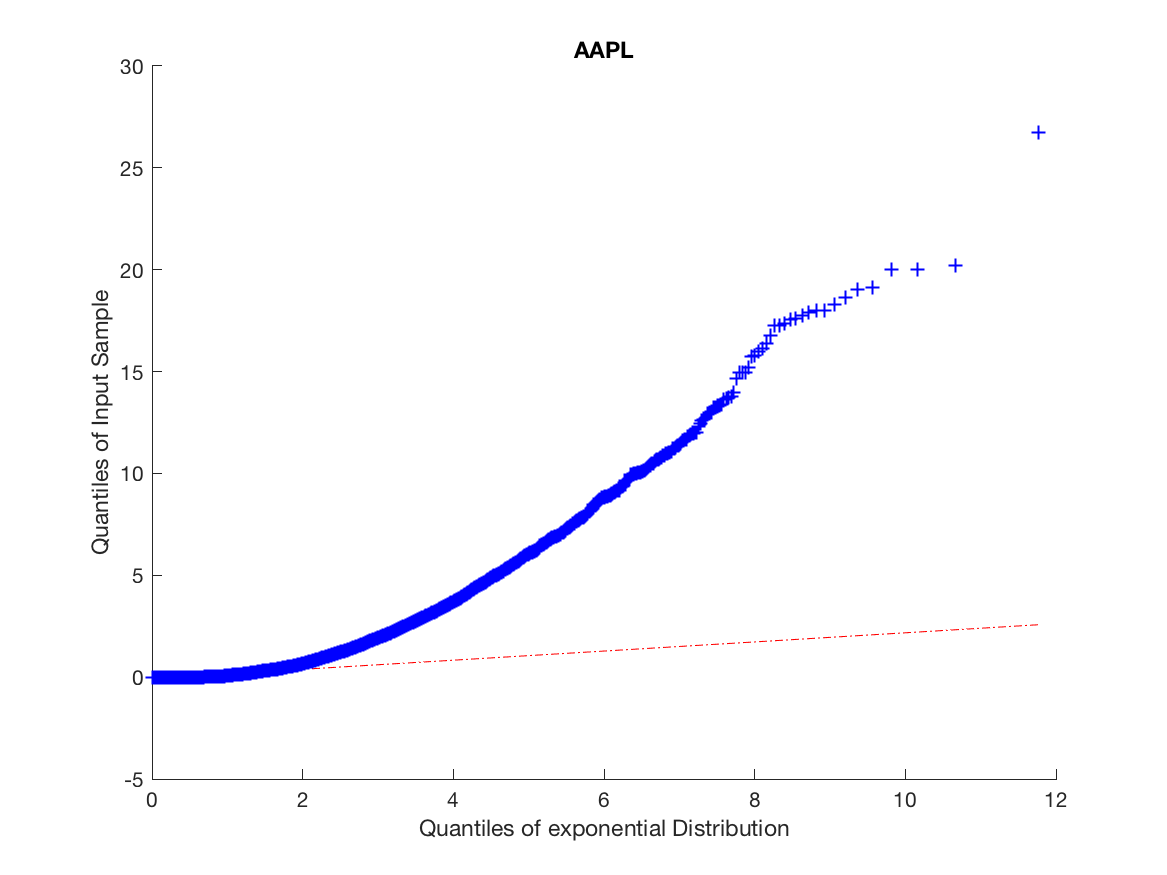
\includegraphics[width=\textwidth, trim = 0 0 0 30, clip]{QQ_Plots/AAPL_QQ.png}

\end{subfigure}
\begin{subfigure}[t]{0.49\textwidth}
\captionsetup{labelformat=empty}

\caption{\textbf{AMZN}}
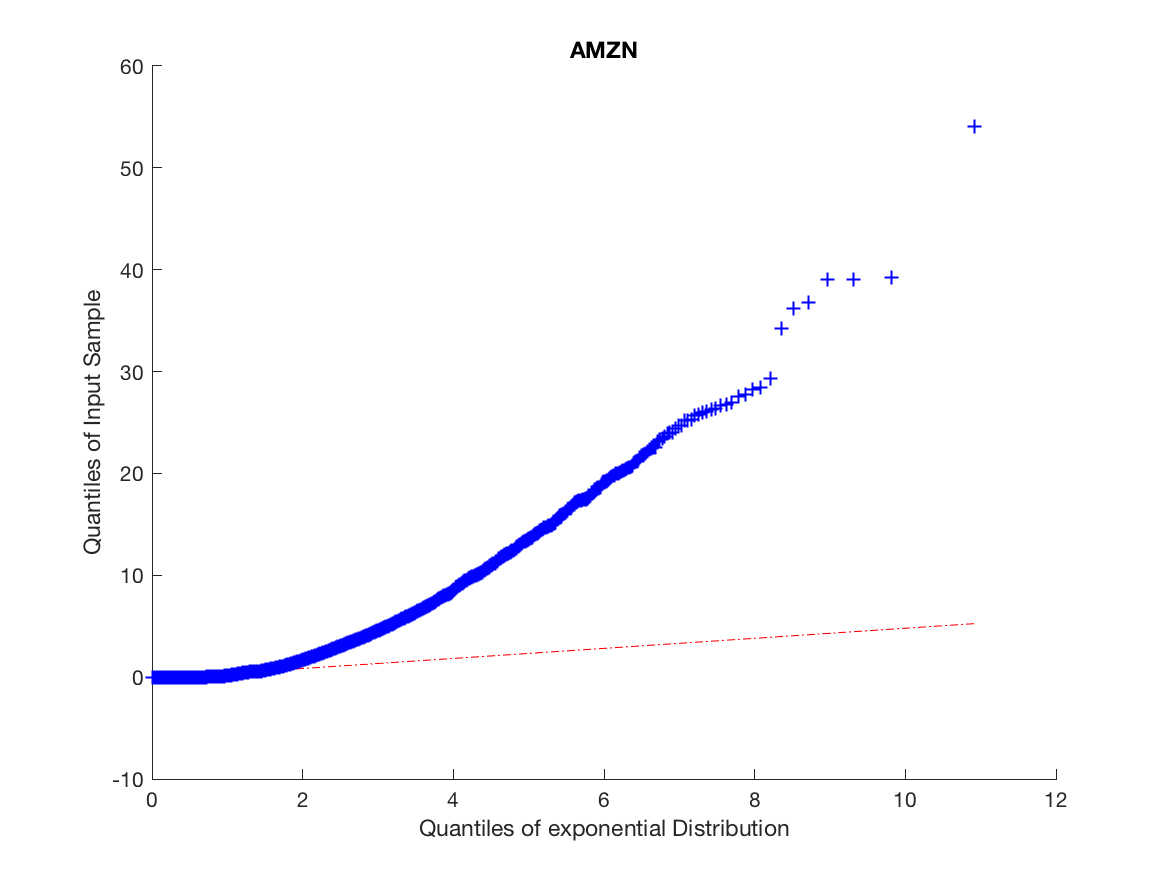
\includegraphics[width=\textwidth, trim = 0 0 0 30, clip]{QQ_Plots/AMZN_QQ.png}
\end{subfigure}

\vspace{3mm}

\begin{subfigure}[t]{0.49\textwidth}
\captionsetup{labelformat=empty}

\caption{\textbf{GOOG}}
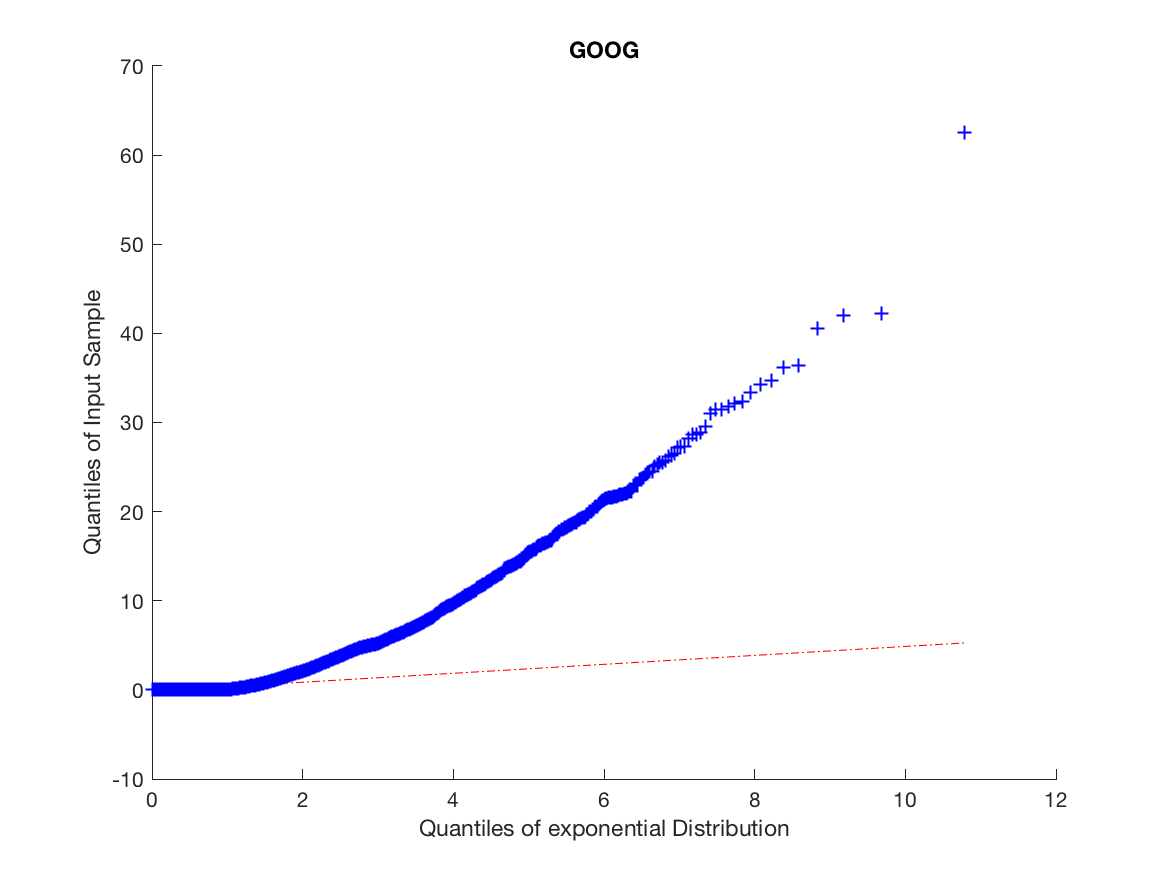
\includegraphics[width=\textwidth, trim = 0 0 0 30, clip]{QQ_Plots/GOOG_QQ.png}

\end{subfigure}
\begin{subfigure}[t]{0.49\textwidth}
\captionsetup{labelformat=empty}

\caption{\textbf{INTC}}
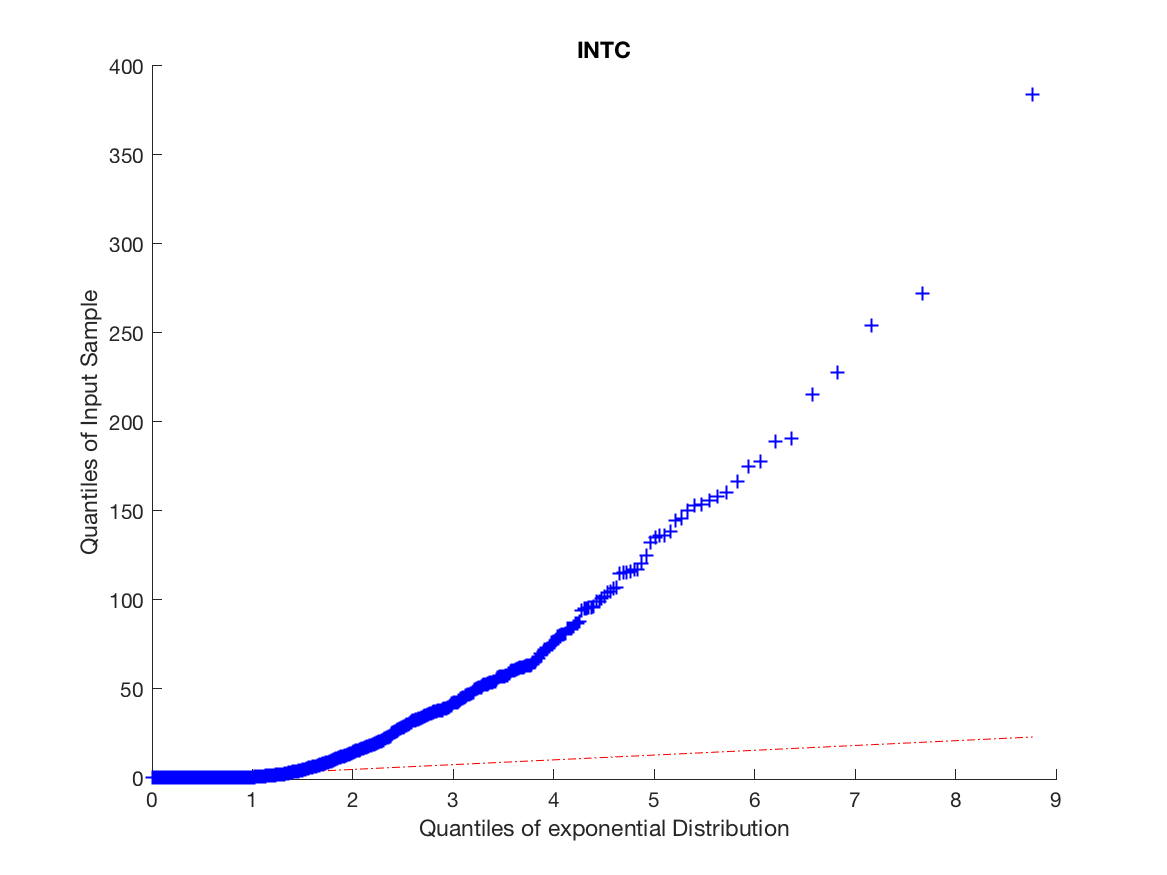
\includegraphics[width=\textwidth, trim = 0 0 0 30, clip]{QQ_Plots/INTC_QQ.png}
\end{subfigure}

\vspace{3mm}

\begin{subfigure}[t]{0.49\textwidth}
\captionsetup{labelformat=empty}

\caption{\textbf{MSFT}}
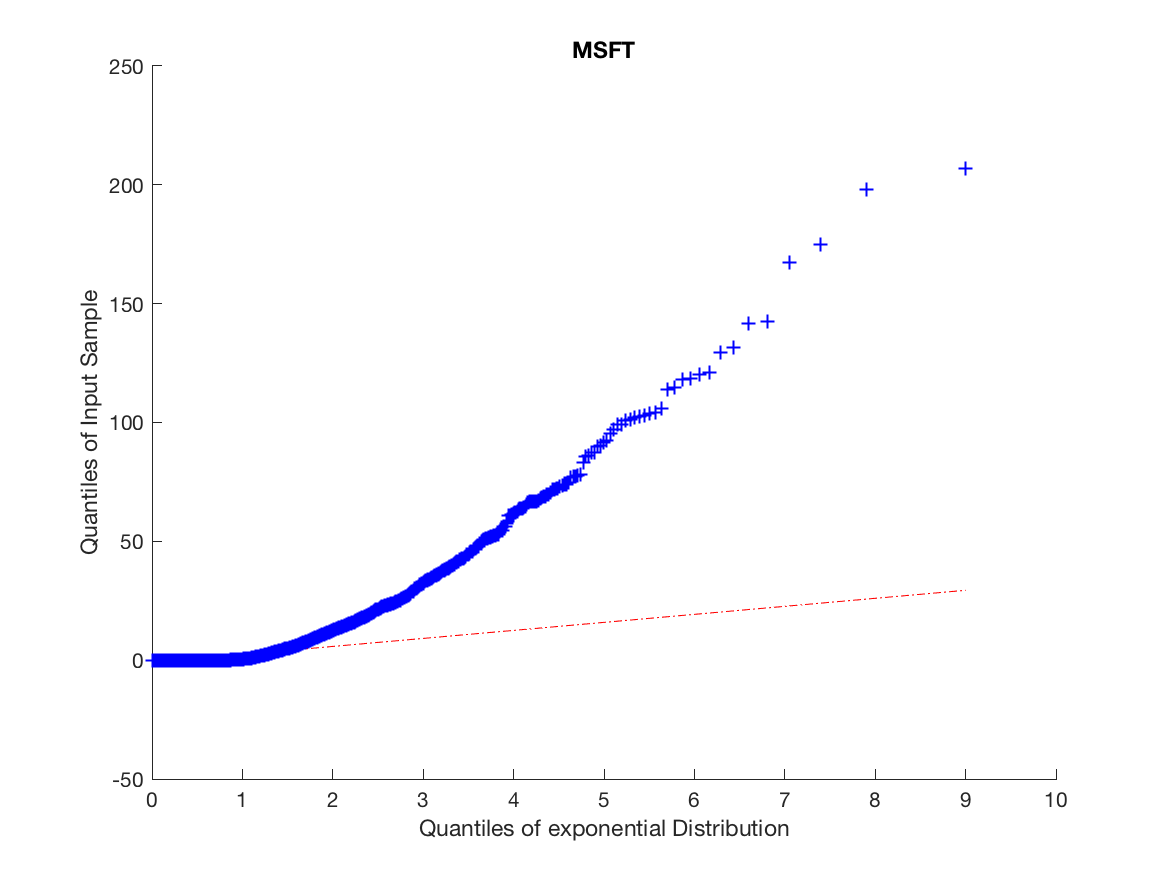
\includegraphics[width=\textwidth, trim = 0 0 0 30, clip]{QQ_Plots/MSFT_QQ.png}
\end{subfigure}

\caption{\label{fig:poisson} Above we provide a quantile-quantile plot of our empirical inter-arrival times against a Poisson process for each of the five stocks. We see that the inter-arrival data does not fit the expected curve, providing evidence that the underlying arrival process is not Poisson.}
\end{figure}